%%%%%%%%%%%%%%%%%%%%%%%%%%%%%%%%%%%%%%%%%%%%%%%%%%%%%%%%%%%%%%%%%%%%%
%%%%%%%%%%%                   PROBLEM 3                   %%%%%%%%%%%
%%%%%%%%%%%%%%%%%%%%%%%%%%%%%%%%%%%%%%%%%%%%%%%%%%%%%%%%%%%%%%%%%%%%%

\section{پرسش سوم}
هر یک از مفاهیم مورد سوال را توضیح می‌دهیم:
\begin{enumerate}[i]
\item \textbf{مرغ و خوک (جلسه‌ی روزانه‌ی اسکرام)} \newline
در جلسه‌ی روزانه‌ متودولوژی scrum افراد حاضر در جلسه را به دو دسته تقسیم می‌کنند. دسته‌ی pigs و دسته‌ی chickens افراد دسته‌ی pigs افرادی اند که کاملا درگیر پروژه و مسئول خروجی و نتیجه‌ی آن هستند و افراد دسته‌ی ‌chickens افرادی اند که در پروژه و جلسات آن شرکت می‌کنند، به صورت مستقیم درگیر پروژه نیستند و پیشرفت و اخبار آن را دنبال می‌کنند.

افراد دسته‌ی pigs افراد اصلی جلسه هستند و در آن به بحث و تبادل اطلاعات می‌پردازند و افراد دسته‌ی chickens تنها شنونده‌ی جلسه اند و نباید در روند آن دخالت کنند.

در یک پروژه‌ی scrum  ، تیم توسعه، 
\lr{Product Owner}
و
\lr{Scrum Master}
افراد دسته‌ی pigs محسوب می‌شوند. در مقابل  ذی‌دفعان، مشتریان و مدیریت اجرایی، افراد گروه chickens هستند.

علت این نامگذاری این است که در یک خوراک تخم‌مرغ و کالباس (پروژه‌ی نرم افزاری) درگیری خوک معادل زندگی اوست و درگیری مرغ (ارائه‌ی تخم مرغ)  امری غیر حیاتی است.

این داستان و نامگذاری از سال ۲۰۱۱ از فرایند رسمی scrum حذف شده است.

\cite{the-chicken-and-the-pig}

\item \textbf{\lr{Burn (down) chart} (اسکرام)} \newline
نمودار Burndown در متودولوژی scrum ابزاری برای تصویر سازی نرخ توسعه‌ی سیستم توسط تیم نرم‌افزاری در برابر نرخ پیش‌بینی شده برای توسعه است تا بتوان به کمک آن تخمینی مناسب از زمان تحویل محصولات پروژه به دست آورد و برای تحویل به موقع آنها برنامه‌ریزی کرد.

در این نمودار تعداد 
\lr{User Story}
‌های پیاده سازی شده در انتهای هر sprint مورد شمارش قرار گرفته و گزارش می‌شود. شمارش
\lr{User Story}
های ناقص اکیدا ممنوع است.

معمولا پس از چند sprint سرعت متوسط توسعه‌ی تیم قابل ارزیابی است و می‌توان تخمینی برای موعد اتمام 
\lr{User Story}
های موجود در backlog ارائه کرد. اگرچه 
backlog
با پیشرفت پروژه دستخوش تغییرات خواهد شد و 
\lr{User Story}
هایی از آن کم و به آن اضافه خواهند شد.



\begin{center}
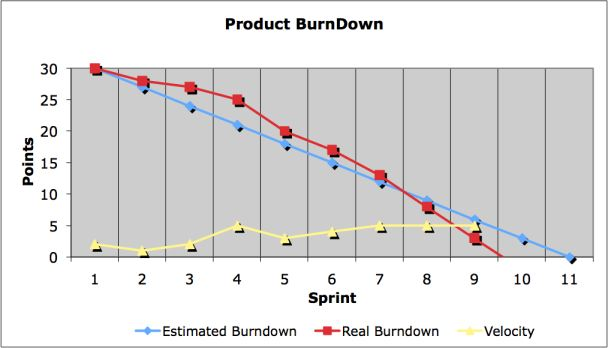
\includegraphics[width = 0.8\textwidth]{images/Simple_Burndown_Chart}

نمودار Burndown ساده - منبع تصویر:
\lr{Scrum Institute}
\LTRfootnote{\url{https://www.scrum-institute.org/Burndown_Chart.php}}
\end{center}


در نمودار Burndown  ساده سرعت تیم توسعه و تغییرات دامنه‌ی پروژه از هم قابل تفکیک نیستند. برای تفکیک این دو از هم از نمودار 
\lr{Extended Burndown}
استفاده می‌شود.
در این نمودار اندازه‌ی هر ستون متناسب با اندازه‌ی backlog در شروع sprint است و تغییرات scope در پایین هر ستون بازتاب می‌یابد.
\cite{burn-down-chart}


\begin{center}
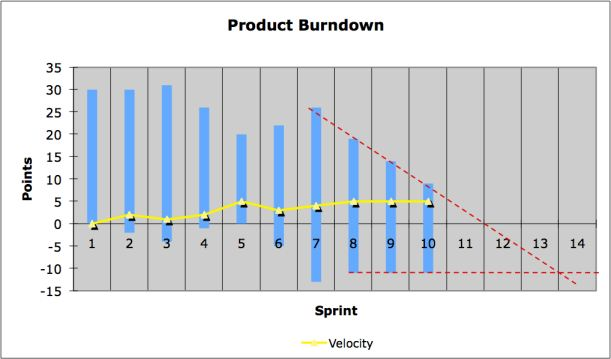
\includegraphics[width = 0.8\textwidth]{images/Extended_Burndown_Chart_with_Prediction}

نمودار \lr{Extended Burndown} به همراه پیشبینی روند توسعه - منبع تصویر:
\lr{Scrum Institute}
\RTLfootnote{همان}
\end{center}

\item \textbf{فاز‌های ترتیبی و فاز‌های تکراری (DSDM)} \newline
یک پروژه‌ی DSDM از ۳ فاز اصلی تشکیل شده است که به صورت ترتیبی اجرا می‌شوند:
\begin{enumerate}[I]
\item \textbf{فاز اول:‌\lr{The Pre-Project}} \newline
در این فاز پروژ‌های کاندیدا مورد بررسی قرار گرفته، تامین مالی پروژه مورد بررسی واقع می‌شود و مسئولیت‌ها در پروژه تعیین می‌شوند.  این موارد باید در ابتدای فرایند پروژه مورد بررسی قرار بگیرند تا از مشکلات آتی پیشگیری شود.

\item \textbf{فاز دوم:‌\lr{The Project life-cycle}} \newline
این فاز ۵ گامی را تببین می‌کند که تیم توسعه باید طی کند تا سیستم نرم‌افزاری ایجاد شود. دو گام اول گام‌هایی ترتیبی هستند و سه گام پس از آنها گامهایی هستند که به صورت Iterative اجرا می‌شوند تا روند ایجاد سیستم تکمیل گردد.

\begin{enumerate}[1]
\item \lr{Feasibility Study}
\item \lr{Business Study}
\item \lr{Functional Model Iteration}
\item \lr{Design and Build Iteration}
\item \lr{Implementation}
\end{enumerate}

\item \textbf{فاز سوم:‌\lr{Post-project}} \newline
در این فاز کارایی درست و بهینه‌ی سیستم مورد ارزیابی و اطمینان قرار می‌گیرد. به این منظور باید از سیستم نگهداری شده و مشکلات آن برطرف شوند. فاز نگهداری را می‌توان ادامه‌ی فاز توسعه‌ی سیستم در متودولوژی DSDM در نظر گرفت.
\cite{dsdm-stages}
\end{enumerate}

\begin{center}
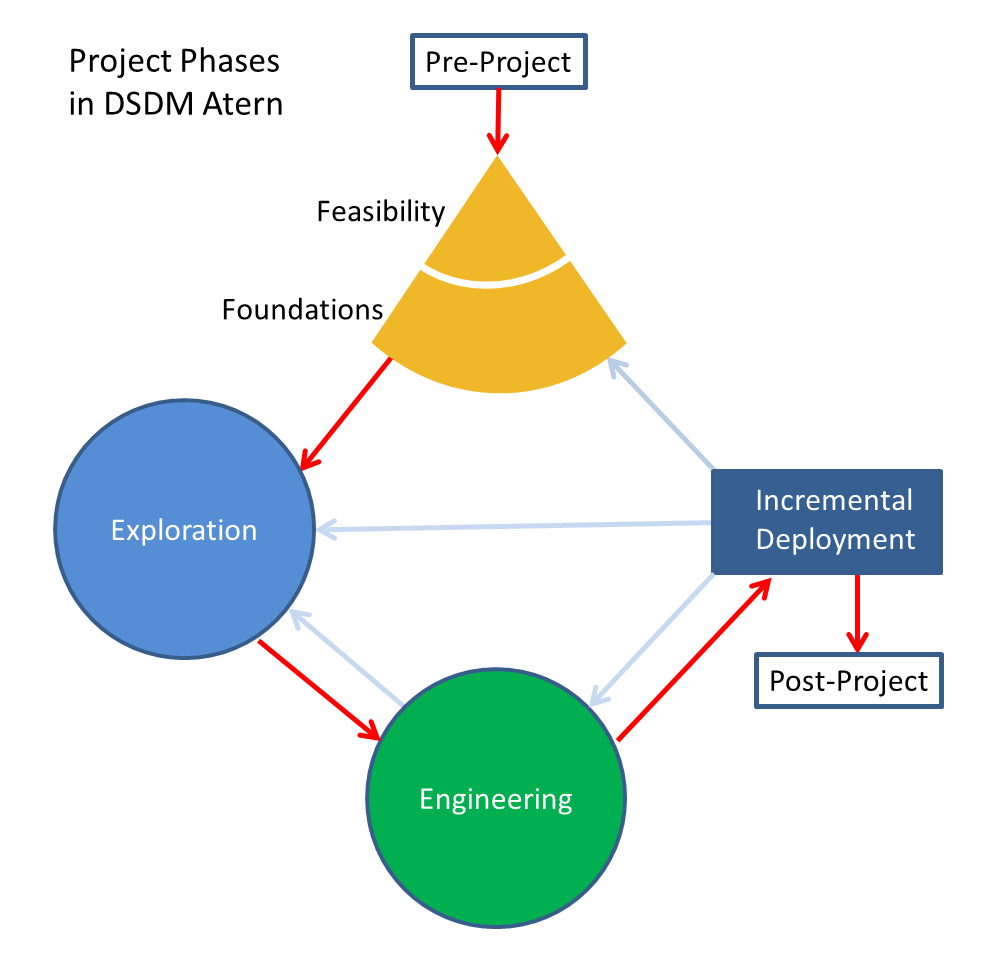
\includegraphics[width = 0.7\textwidth]{images/DSDM_Atern_Project_Phases}

گام‌های توسعه در متودولوژی DSDM - منبع تصویر:
\lr{Wikipedia}
\LTRfootnote{\url{https://en.wikipedia.org/wiki/File:DSDM_Atern_Project_Phases.png}}
\end{center}

\item \textbf{محیط مالکیت تجمعی کد (XP)} \newline
مالکیت تجمعی کد هر گونه مالکیت فردی یا خصوصی بر روی کد یا ماژول‌ها را در یک محیط توسعه‌ی تیمی نادیده می‌گیرد. مالکیت منابع کد با کل تیم توسعه‌ی نرم‌افزاری است و هر فرد می‌تواند در صورت نیاز برای پیاده سازی بخشی از نیازمندی‌ها هر بخشی از کد را که بخواهد تغییر دهد.

این مفهوم مالکیت تیمی را در مقابل مالکیت شخصی بر روی کد نوشته شده قرار می‌دهد.

این مفهوم از متودولوژی XP
\LTRfootnote{eXtreme Programming}
 گرفته شده است و در مقابل مفهوم 
\lr{Class Ownership}
در متودولوژی FDD
است.
\cite{code-ownership}

\item \textbf{کارگاه تفکر (بازتاب) (Crystal)} \newline
بهبود بازتابی
\LTRfootnote{Reflective improvement}
به فرایندی گفته می‌شود که در آن توسعه دهندگان سیستم نرم‌افزاری برای مدتی دست از توسعه‌ی سیستم کشیده و تلاش می‌کنند راه‌هایی برای بهبود فرایند‌های مورد استفاده‌شان در تولید نرم‌افزار پیدا کنند.

می‌توان با دقت در چرخه‌های تولید نرم‌افزار متوجه شد که آیا فرایند‌های فعلی دارای مشکلاتی هستند یا نه.

در خانواده‌ی متودولوژی‌های Crystal تیم‌های نرم‌افزاری به برگزاری جلسات دو‌هفتگی کارگاه تفکر بازتاب تشویق شده‌اند. در این جلسات فرایند‌های تیم مورد بررسی قرار می‌گیرند تا فرایند‌هایی که خوب کار می‌کنند و فرایند‌هایی که به علت مشکلات نیاز به تغییرات دارند شناسایی شوند. به این ترتیب این فرایند‌ها به تدریج در جهت منافع تیم تغییر خواهند کرد.
\cite{reflective-workshop}

\end{enumerate}
